\documentclass[letterpaper,12pt]{scrartcl}
\usepackage{epsfig,latexsym,amsmath,amssymb,epic,eepic,psfrag,subfigure,float,euscript,array}
\usepackage[latin1]{inputenc}
\usepackage[margin=24mm]{geometry}
\usepackage{enumitem}
\usepackage{tikz,pgf,pgfplots}
\usepgfplotslibrary{fillbetween}
\usetikzlibrary{decorations, arrows}

\usepackage[amssymb]{SIunits}

\newenvironment{exercise}[1][Uppgift]{\begin{trivlist} \item[\hskip
    \labelsep {\stepcounter{exerctr}\bfseries #1
      \arabic{exerctr}}]}{\end{trivlist}\vspace{10mm}}

\newcounter{exerctr}
\newcounter{abcctr}[exerctr]

\newcommand{\abc}{\noindent\vspace{1mm}\\ {\bf
    \stepcounter{abcctr}(\alph{abcctr})\ }}
\newcommand{\bbm}{\begin{bmatrix}}
\newcommand{\ebm}{\end{bmatrix}}
\newcommand{\point}[1]{\hfill {\bf (#1p)}\\ \vspace{-5mm}}
\newcommand{\ctrb}{\EuScript{S}}
\newcommand{\Lap}{\mathcal{L}}
\newcommand{\obsv}{\EuScript{O}}
\newcommand{\realdel}{\text{Re}}
\newcommand{\imagdel}{\text{Im}}
\newcommand{\bC}{\mathbb{C}}
\newcommand{\bR}{\mathbb{R}}
\newcommand{\bmpv}{\begin{minipage}[t]}
\newcommand{\bmps}{\begin{minipage}[t]{45mm}}
\newcommand{\bmpm}{\begin{minipage}[t]{90mm}}
\newcommand{\bmpl}{\begin{minipage}[t]{\textwidth}}
\newcommand{\emp}{\end{minipage}}
\newcommand{\mexp}[1]{\ensuremath{\mathrm{e}^{#1}}}
\newcommand*{\laplaceinv}[1]{\ensuremath{\mathcal{L}^{-1} \left\{#1\right\}}}
\newcommand*{\ztrf}[1]{\ensuremath{\mathcal{Z} \left\{#1\right\}}}

\newcommand{\AxisRotator}[1][rotate=0]{%
    \tikz [x=0.2cm,y=0.60cm,line width=.1ex,-stealth,#1] \draw (0,0) arc (-150:150:1 and 1);%
}

\newcommand{\shift}{\ensuremath{\operatorname{q}}}
%\addtolength{\topmargin}{-1cm}
%\textheight 22.5cm
%\oddsidemargin 1.3cm
%\evensidemargin 1.3cm

\makeatletter
\newcommand*{\rom}[1]{\expandafter\@slowromancap\romannumeral #1@}
\makeatother

\newcommand*\circled[1]{\tikz[baseline=(char.base)]{
            \node[shape=circle,draw,inner sep=2pt] (char) {#1};}}


\title{Computerized Control partial exam 1 (15\%)}
\author{Kjartan Halvorsen}
\date{}

\begin{document}

\maketitle


\begin{description}
\item[Time] February 13 17:35-18.55
\item[Place] 5105
\item[Permitted aids] The single colored page with your own notes, table of Laplace transforms, calculator
\end{description}

All answers should be readable and well motivated (if nothing else is written). Solutions/motivations should be written on the provided spaces in this exam. Use the last page if more space is needed.

\begin{center}
{\Large Good luck!} \\
\end{center}

\noindent
\fbox{
\bmpl
{\bf Matricula and name:}\\
\vspace*{14mm}
\emp}


%\clearpage

%-----------------------------------------------------------------

\subsection*{Flow control in a valve}
A butterfly valve is used to control the flow of petroleum in an oil refinery. The valve is a so-called quarter-turn valve, and goes from fully closed $\theta=\unit{0}{\degree}$ to fully open  in a quarter rotation of the valve shaft $\theta=\unit{90}{\degree}$. The valve shaft is actuated by a DC motor via a transmission (gear box).
% with the ratio 30:1 (\unit{30}{\degree} rotation of the shaft of the DC motor gives \unit{1}{\degree} rotation of the valve shaft) 
\begin{center}
  \begin{tikzpicture}[node distance=20mm]
    \node (image) {\includegraphics[width=0.16\textwidth]{../../../MR2012/figures/butterfly-valve-servo-motor.jpg}};

    \def\tubelength{15mm}
    \def\tubewidth{4mm}
    \def\tuberad{2mm}
    \def\valvelength{3mm}

    \begin{scope}[xshift=5cm, yshift=-1cm]
     \draw (0,0) -- (\tubelength, 0);
     \draw (0,\tubewidth) -- (\tubelength, \tubewidth);
     \draw (\tubelength, 0) -- ++(\valvelength, \tuberad) node[coordinate, at end] (valve) {};
     \draw (\tubelength, \tubewidth) -- ++(\valvelength, -\tuberad);
     \draw (valve) -- ++(\valvelength, \tuberad);
     \draw (valve) -- ++(\valvelength, -\tuberad);
     \draw (valve) ++(\valvelength, \tuberad) -- ++(\tubelength, 0);
     \draw (valve) ++(\valvelength, -\tuberad) -- ++(\tubelength, 0);

     \node[rectangle, draw, minimum height=6mm, minimum width=8mm, above of=valve, node distance=16mm] (box) {};
     
     \draw[-o] (box.north) ++(-2mm, 0) -- ++(0,4mm);
     \draw[-o] (box.north) ++(2mm, 0) -- ++(0,4mm);

     \node[above of=box, node distance=10mm] {$u(t)$};

     \draw[ultra thick] (box) -- node[midway] {\AxisRotator[rotate=90]} node[left, pos=0.24] {$\theta$} (valve);

     \draw[->, thick] (valve) ++(12mm,0) -- node[near end, anchor=south west] {$Q(t) = Q_0 + y(t)$} ++(10mm,0);
   \end{scope}
 \end{tikzpicture}
\end{center}
The signal $u(t)$ [\unit{}{\volt}] is the voltage over the DC motor and the signal $Q(t)$ [\unit{}{\meter\cubed\per\second}] is the flow through the valve.

\subsection*{Problem 1}

In order to use methods for discrete-time control you need to determine a discrete model of the plant. In continuous time the dynamical system from the input signal $u(t)$ to the angle of the valve shaft $\theta(t)$ is well described by the transfer function
\[ \Theta (s) = \frac{k_V}{s(sT_V + 1)} U(s). \]
Sample the system using zero-order-hold. You can make use of the partial fraction expansion
\[ \frac{k_V}{s^2(sT_V+1)} = k_V \left( \frac{1}{s^2} - \frac{T_v}{s} + \frac{T_V^2}{sT_V + 1} \right).\]

\noindent
\fbox{
\bmpl
{\bf Calculations:}\\
\vspace*{15cm}
\emp}

\subsection*{Problem 2}

  The flow through the valve depends on the product of the valve angle $\theta$ and the square root of the pressure difference $\Delta P = P_u - P_d$ across the valve
  \[ Q(t) = k_\theta \theta(t) \sqrt{\Delta P(t)} = f\big(\theta(t), \Delta P(t)\big),\]
 where  $k_\theta$ is a positive constant. Defining deviations around an operating point $\Delta P(t) = \Delta P_0 + v(t)$, $\theta(t) = \theta_0 + \phi(t)$, the nonlinear model of the flow can be linearized. In suitable units, the linear discrete model of a specific, electrically actuated butterfly valve can be represented by the block-diagram below
\begin{center}
  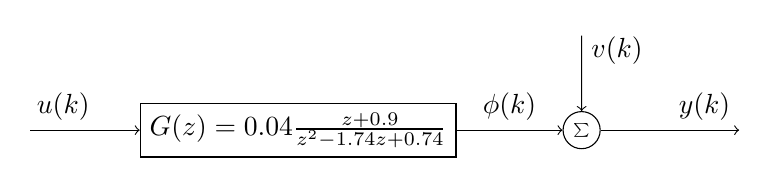
\begin{tikzpicture}[scale = 0.8, node distance=22mm, block/.style={rectangle, draw, minimum width=15mm}, sumnode/.style={circle, draw, inner sep=2pt}]
    
    \node[coordinate] (input) {};
     \node[block, right of=input, node distance=34mm] (valve) {$G(z)=0.04\frac{z+0.9}{z^2 - 1.74z + 0.74}$};
     \node[sumnode, right of=valve, node distance=36mm] (sum) {\tiny $\sum$};
     \node[coordinate, right of=sum, node distance=20mm] (output) {};
     \node[coordinate, above of=sum, node distance=12mm] (disturbance) {};

     \draw[->] (input) -- node[above, pos=0.3] {$u(k)$} (valve);
     \draw[->] (valve) -- node[above] {$\phi(k)$} (sum);
     \draw[->] (sum) -- node[above, near end] {$y(k)$} (output);
     \draw[->] (disturbance) -- node[right, pos=0.2] {$v(k)$} (sum);
   \end{tikzpicture}
   \end{center}

You are aware of the fact that the pressure in the pipe can vary, so you consider using a feedback controller in order to try to keep the flow through the valve constant even in the presence of changes in the pressure. A flow meter is installed that measures the flow $Q(t)$. By subtracting the operating point value $Q_0$, the sampled signal $y(k) = Q(k) - Q_0$ is available for feedback control. 

\begin{center}
  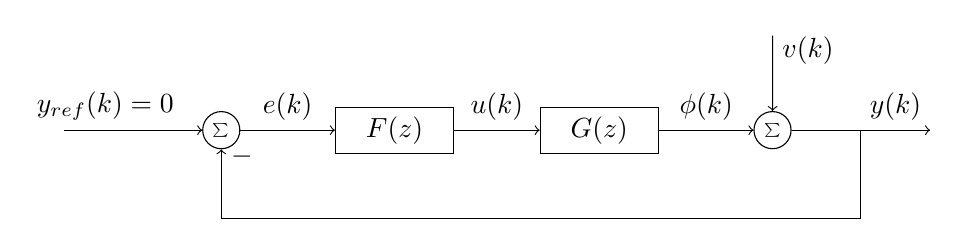
\begin{tikzpicture}[scale = 0.8, node distance=22mm, block/.style={rectangle, draw, minimum width=15mm}, sumnode/.style={circle, draw, inner sep=2pt}]
    
    \node[coordinate] (refinput) {};
     \node[sumnode, right of=refinput, node distance=20mm] (sumerr) {\tiny $\sum$};
     \node[block, right of=sumerr] (controller) {$F(z)$};
     \node[block, right of=controller, node distance=26mm] (valve) {$G(z)$};
     \node[sumnode, right of=valve, node distance=22mm] (sum) {\tiny $\sum$};
     \node[coordinate, right of=sum, node distance=20mm] (output) {};
     \node[coordinate, above of=sum, node distance=12mm] (disturbance) {};

     \draw[->] (controller) -- node[above] {$u(k)$} (valve);
     \draw[->] (valve) -- node[above] {$\phi(k)$} (sum);
     \draw[->] (sum) -- node[coordinate] (measure) {} node[above, near end] {$y(k)$} (output);
     \draw[->] (disturbance) -- node[right, pos=0.2] {$v(k)$} (sum);

     \draw[->] (refinput) -- node[above, pos=0.3] {$y_{ref}(k)=0$} (sumerr);
     \draw[->] (sumerr) -- node[above] {$e(k)$} (controller);

     \draw[->] (measure) -- ++(0,-14mm) -| node[right, pos=0.95] {$-$} (sumerr);
     \end{tikzpicture}
   \end{center}

\subsubsection*{(a)}


Determine the closed-loop pulse transfer function from the pressure disturbance $v(k)$ to the output signal (flow deviation) $y(k)$. 

\noindent
\fbox{
\bmpl
{\bf Calculations:}\\
\vspace*{8cm}
\emp}

 
\subsubsection*{(b)}
As a good engineer, you try the simplest solution first and test if that is good enough. So, you try a proportional controller $F(z) = K$. The  root-locus below shows how the closed-loop poles depend on the controller gain $K$. Describe in words (3-5 sentences) some interesting properties (stability, damping, speed) of the system that the root locus below tells us as the gain $K$ varies from 0 to $\infty$.
\begin{center}
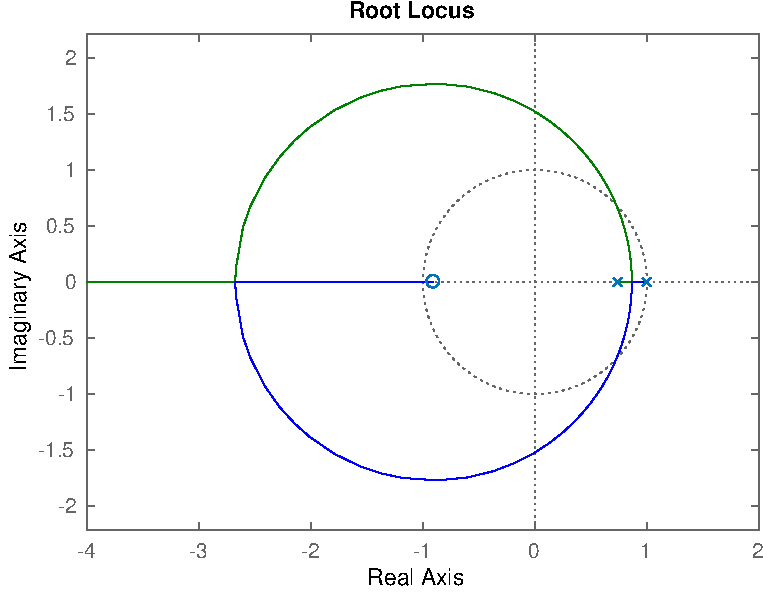
\includegraphics[width=0.5\linewidth]{root-locus-crop}
\end{center}

\noindent
\fbox{
\bmpl
{\bf Description:}\\
\vspace*{6cm}
\emp}

\subsubsection*{(c)}
With the gain $K=1$, the next Bode diagram is obtained for the loop gain $G_o(z) = KG(z)$. Determine and indicate in the diagram (draw) the 
\begin{enumerate}[itemsep=0mm]
\item cross-over frequency
\item phase margin
\item phase cross-over frequency
\item amplitude margin
\end{enumerate}

\noindent
\fbox{
\bmpl
%\begin{center}
\hfill
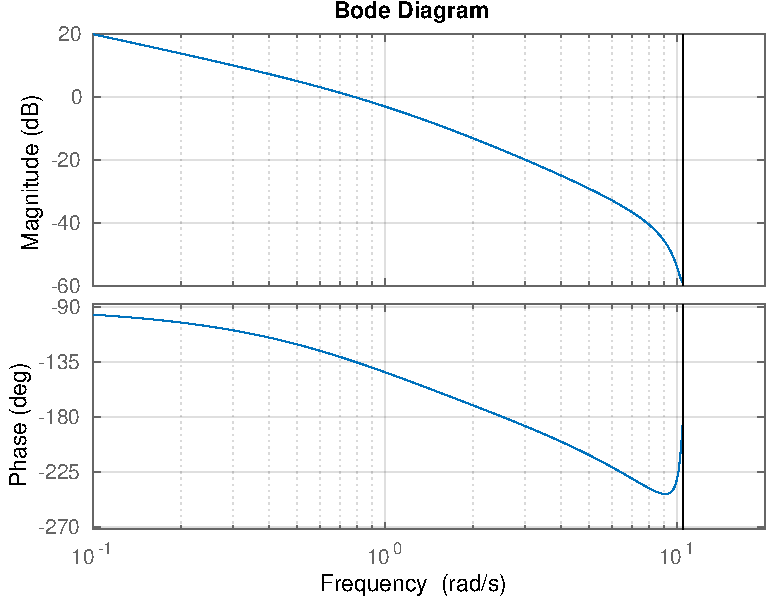
\includegraphics[width=0.6\linewidth]{bode-diagram-crop}
%\end{center}
\emp}

\noindent
Bonus question (worth 5p):

\noindent
\fbox{
\bmpl
What is the sampling period of the discrete-time system? Motivate!
\vspace*{15mm}
\emp}


\subsubsection*{(d)}
You find it difficult to achieve the desired performance for the closed-loop system with a simple proportional controller. So, instead you try a lead-compensator
\[ F(z) = K \frac{z-b}{z-a}, \qquad b>a. \]
Why would a lead-compensator give better performance than the proportional controller in this case?

\noindent
\fbox{
\bmpl
{\bf Answer:}\\
\vspace*{4cm}
\emp}

\subsubsection*{(e)}
The lead-compensator in (d) can be written \[U(z) = F(z)E(z) \quad \text{or} \quad u(k) = F(q) e(k).\] 
Write the lead-compensator as a difference equation, so that it can be implemented on a microcontroller.

\noindent
\fbox{
\bmpl
{\bf Calculations:}\\
\vspace*{6cm}
\emp}

%\cleardoublepage%
%\end{document}
\section*{Solutions}
\subsection*{Problem 1}
We first need to determine the step response of the continous-time system.
\begin{equation*}
\begin{split}
 \theta(t) &= \laplaceinv{\frac{k_V}{s(sT_V+1)} \cdot \frac{1}{s}} = k_V \left( \laplaceinv{\frac{1}{s^2}} - \laplaceinv{\frac{T_V}{s}} + \laplaceinv{\frac{T_V^2}{sT_V + 1}} \right)\\
 &= k_V \left( t - T_Vu_H(t) + T_V\mexp{-\frac{t}{T_V}}\right).
\end{split}
\end{equation*}
Then sample (set $t=kh$) and apply the z-transform
\begin{equation*}
\begin{split}
\Theta(z) &= k_V \left( \ztrf{kh} -T_V\ztrf{u_H(kh)} + T_V\ztrf{\mexp{-\frac{kh}{T_V}}} \right)\\
&= k_V \left( \frac{zh}{(z-1)^2} - \frac{T_V z}{z-1} + \frac{T_V z}{z - \mexp{-\frac{h}{T_V}}} \right).
\end{split}
\end{equation*}
Divide by the z-transform of the input signal (step) to obtain
\begin{equation*}
\begin{split}
  G(z) &= \frac{\Theta(z)}{U(z)} = k_V\frac{z-1}{z} \left ( \frac{zh}{(z-1)^2} - \frac{T_V z}{z-1} + \frac{T_V z}{z - \mexp{-\frac{h}{T_V}}} \right)\\
&= k_V\left( \frac{h}{z-1} - T_V + \frac{T_V(z-1)}{z - \mexp{-\frac{h}{T_V}}} \right)\\
&= k_V \frac{h(z-\mexp{-\frac{h}{T_V}}) - T_V(z-1)(z-\mexp{-\frac{h}{T_V}}) + T_V(z-1)^2}{(z-1)(z-\mexp{-\frac{h}{T_V}})}.
\end{split}
\end{equation*}

\subsection*{Problem 1}
\subsubsection*{(a)}
The closed-loop system is
\[ Y(z) = V(z) + G(z)F(z)E(z) = V(z) - G(z)F(z)Y(z) \]
so
\[ Y(z) = \frac{1}{1 + G(z)F(z)} V(z)\]
and the desired closed-loop pulse transfer function is
\[ G_c(z) = \frac{1}{1 + G(z)F(z)} = \frac{1}{1 + F(z)0.04\frac{z+0.9}{z^2 - 1.74z + 0.74}}
          = \frac{z^2 - 1.74z + 0.74}{z^2 - 1.74z + 0.74 + F(z)0.04(z+0.9)}. \]

\subsubsection*{(b)}
We see starting points in $z=1$ and $z=0.74$ (the roots of $z^2 - 1.74z + 0.74$). For small $K$ the system will be stable and dominated by the slow pole near $1$. As $K$ increases, the two poles will meet on the real axis. Such a system is critically damped. Further increasing $K$ causes the branches to go out into the complex plane and the system becomes under-damped. The branches break out of the unit circle at some point, and so the system becomes unstable.

\subsubsection*{(c)}
\begin{center}
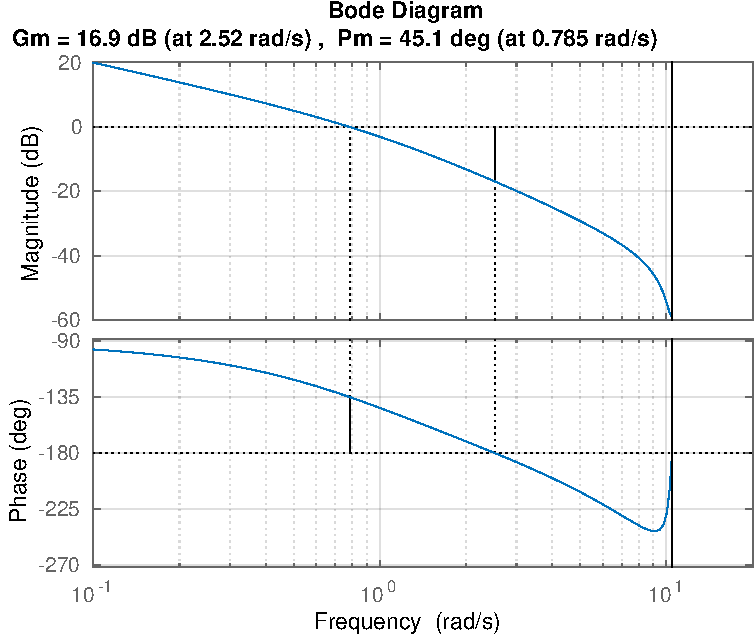
\includegraphics[width=0.6\linewidth]{margin-diagram-crop}
\end{center}

\subsubsection*{(d)}
The lead-compensator moves the branches of the root locus further to the left. This means that it is possible to achieve a closed-loop system with poles that are further from the point 1 and at the same time further inside the unit circle than what is possible with the proportional controller. This gives a faster and more damped closed-loop system.

\subsubsection*{(e)}
We have
\[u(k) = F(q) e(k) = K\frac{\shift - b}{\shift - a}e(k) \]
\[ (\shift - a) u(k) =K (\shift - b) e(k)\]
\[ \shift u(k) - au(k) = K\shift e(k) - Kbe(k)\]
\[ u(k+1) = a u(k) + Ke(k+1) - Kb e(k).\]

\end{document}

